\section{Comportamiento táctico}

% TODO quitar
% Para el funcionamiento del juego hemos diseñado un comportamiento y características propias de cada personaje. Para esto hemos usado una herramienta llamada Behavior Trees \cite{uniBT}, el cual nos permite crear un árbol de decisiones sobre cada unidad. Dentro de estos árboles podemos encontrar distintos nodos. Para poder entender mejor estos árboles de comportamiento primero veremos los Scripts que encontramos dentro  del directorio \directory{Assets/Scripts/Tactica/Behaviour} del proyecto, creados para las acciones y las condiciones que serán la clave del comportamiento `inteligente' de cada personaje.

\subsection{Condiciones}

En total contamos con 13 scripts de condiciones distintos que heredan de la clase \texttt{Conditional} que modelan el comportamiento de nuestros agentes. Estos scripts en el método \texttt{IsUpdatable} se encargan de llamar a los métodos del agente definido que comprueban una condición en especial. Los bloques de código serán tanto del método \texttt{IsUpdatable} cómo de la clase \texttt{AgentNPC} que es la clase padre de todos nuestros personajes, encargada de implementar todos los métodos de comprobación de condiciones a los que se llaman. 

\begin{itemize}
    \item \textbf{Comprobaciones de estado}: para este cometido se tienen 3 nodos distintos. Cada uno comprueba si el estado actual del personaje es ataque (\texttt{AttackMode}), defensa (\texttt{DefenseMode}), o bien, guerra total (\texttt{Total War}).
    \item \textbf{Comprobación de muerte}: esta labor recae sobre un nodo (\texttt{IsAlive}) que comprueba si el agente está vivo. Esta comprobación controla la ejecución del resto del árbol.
    \item \textbf{Comprobaciones de salud}: tenemos dos comprobaciones sobre el estado de salud del personaje. Una de ellas (\texttt{LowHP}) comprueba si la salud del enemigo ha caído por de la mitad de los puntos totales. La otra (\texttt{NotFullHP}) comprueba si un personaje no tiene la totalidad de los puntos de salud.
    \item \textbf{Comprobaciones de localización del personaje}: esta es la categoría donde más nodos distintos hay. Los podemos dividir en 3 grupos, según las distancias que comprueban:
        \begin{itemize}
            \item \textbf{Comprobación de localización exacta}: con estos nodos se comprueba si el personaje está en una estructura concreta. En esta categoría tenemos \texttt{OnHealingPoint} y \texttt{OnEnemyBase}. 
            \item \textbf{Comprobación de cercanía}: en estos nodos se comprueba si el agente está cerca de una estructura. A este categoría pertenecen los nodos \texttt{NearToEnemy Base} y \texttt{NearToTeamBase}.
            \item \textbf{Comprobación de lejanía}: en estos nodos se comprueba si el agente está lejos de una estructura. A este categoría pertenecen los nodos \texttt{FarFromEnemy Base} y \texttt{FarFromTeamBase}.
            
            Tanto para las comprobaciones de lejanía como de cercanía se usa la distancia de Chevychev. 
        \end{itemize}
\end{itemize}

Una vez vista las condiciones veamos las acciones que llevarán a cabo nuestros agentes.

\subsection{Acciones}

En lo que respecta a acciones tenemos 6 scripts distintos que en este caso heredarán de la clase \texttt{Action}. Esta acciones serán los nodos hoja de nuestros árboles de comportamiento, ya que se ejecutarán una vez realizadas todas las comprobaciones sobre las condiciones establecidas. En este caso la implementación de la acción requerida se encuentra en el método \texttt{OnUpdate}, veamos las diferentes implementaciones:

\begin{itemize}
    \item \textbf{Atacar a un enemigo} (\texttt{AttackEnemy}): el agente ataca al enemigo más cercano que esté en su rango de ataque. Estos ataques se producen cada cierto número de segundos, que serán la velocidad de ataque del agente.
    
        \lstinputlisting[linerange=420-443, firstnumber=420]{\ScriptsPath/Steering/NPC/AgentNPC.cs}
    
    \item \textbf{Capturar base enemiga} (\texttt{CaptureEnemyBase}): el agente aporta puntos de captura a la base enemiga mientras se encuentre en ella.
        
        \lstinputlisting[linerange=688-708, firstnumber=688]{\ScriptsPath/Steering/NPC/AgentNPC.cs}
        
    \item \textbf{Curarse} (\texttt{Heal}): el agente obtiene puntos de salud del punto de curación. Estos puntos de salud se recuperan en forma de pulsos cada cierto tiempo.
        
        \lstinputlisting[linerange=535-560, firstnumber=535]{\ScriptsPath/Steering/NPC/AgentNPC.cs}
        
    \item \textbf{Ir a una estructura}: el agente se dirige hacia una estructura como la base enemiga (\texttt{GoToEnemyBase}), su propia base (\texttt{Defend}) o el punto de curación (\texttt{GoHealing}).
    
        \lstinputlisting[linerange=356-371, firstnumber=356]{\ScriptsPath/Steering/NPC/AgentNPC.cs}
\end{itemize}


\subsection{Comportamiento de los agentes}
Ahora que ya hemos visto cómo serían todos los elementos del comportamiento táctico de los personajes, podemos ver cómo se han juntado todos estos elementos para crear los árboles de comportamiento de los distintos tipos de unidades.
\subsubsection{Infantería}
Esta unidad la hemos interpretado con una máxima prioridad sobre ganar la partida. Priorizará capturar la base enemiga sobre cualquier cosa. En \textbf{modo ataque} la unidad prioriza capturar la base enemiga sobre todas las cosas, seguido de atacar a los enemigos. Y después pensará en su salud, pero solo cuando no pueda capturar o atacara a un enemigo. En\textbf{ modo defensa} defenderá atacando a los enemigos que vea y no pensará en curarse. Por ultimo, en \textbf{modo guerra total} se actuará como en ataque pero sin pensar en curarse.

\begin{figure}[H]
    \centering
    \resizebox{0.9\textwidth}{!}{
        \begin{tikzpicture}
            \node (0) {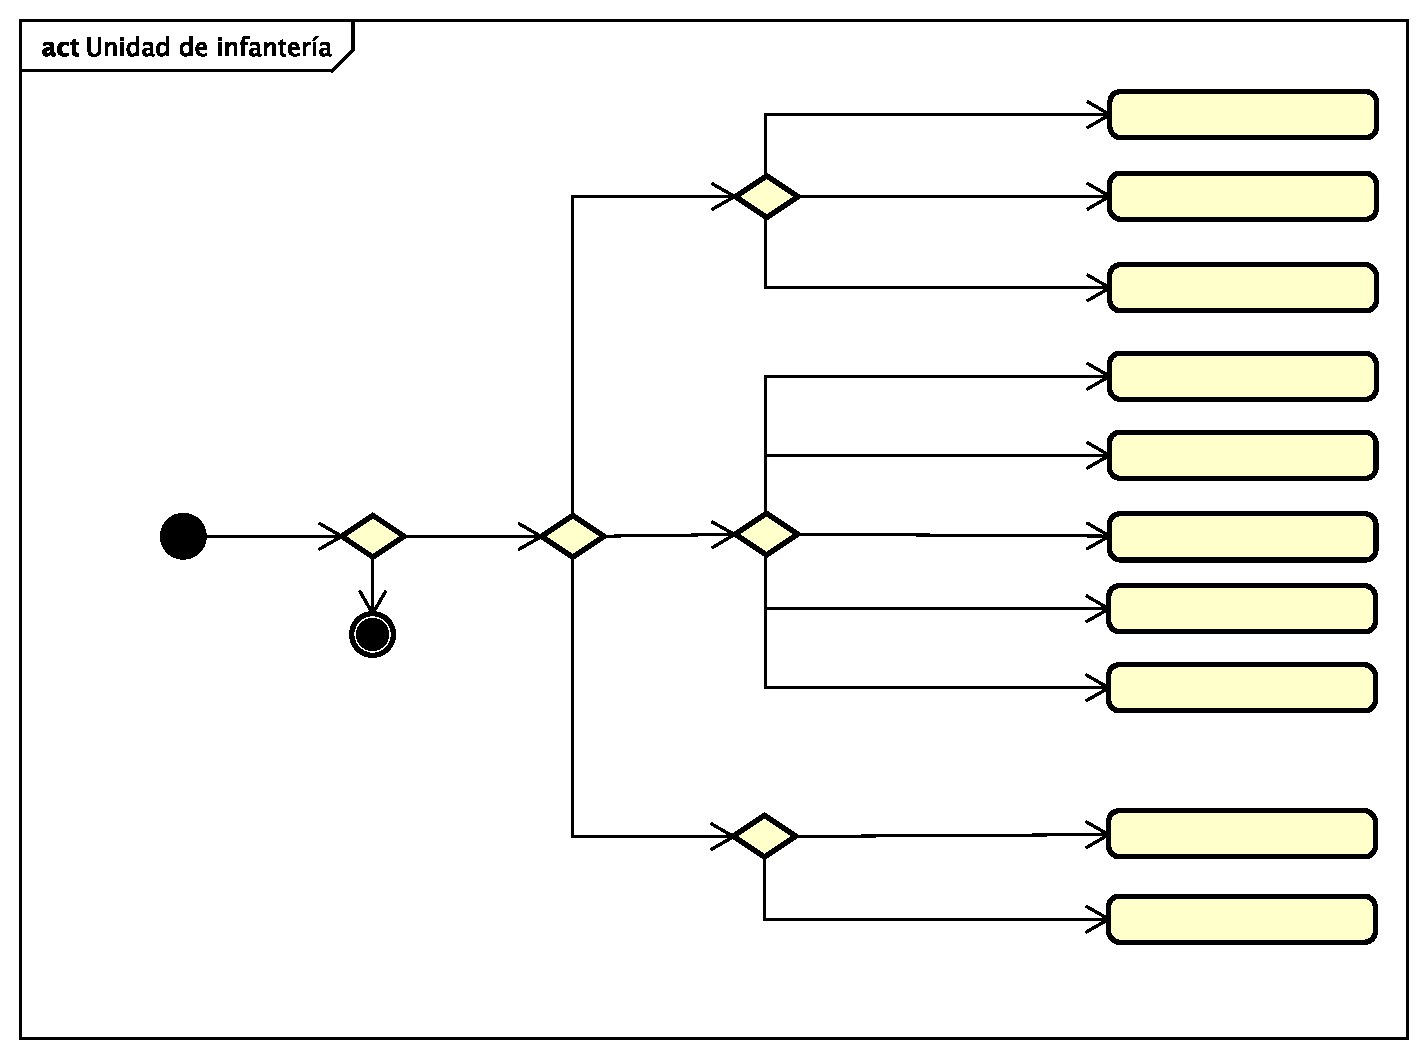
\includegraphics{behaviourTrees/pdfs/arbolInfanteria}};
            \node (1) at (-6.3,-0.75) {No};
            \node (2) at (-4.9,0.2) {Sí};
            \node (3) at (-6.5,0.3) {¿Vivo?};
            \node (4) at (-3.3,0.4) {¿Estado?};
            \node (5) at (-1.3,6) {Guerra Total};
            \node (6) at (-1.3,0.2) {Ataque};
            \node (7) at (-1.3,-4.9) {Defensa};
            
            \node (8) at (3,6) {¿Enemigo cerca?};
            \node (9) at (3,7.3) {¿En base enemiga?};
            \node (10) at (9,5.6) {Atacar enemigo};
            \node (11) at (9,7) {Capturar base enemiga};
            \node (12) at (9,4.1) {Ir a la base enemiga};
            
            \node (13) at (3,1.6) {¿Enemigo cerca?};
            \node (14) at (3,2.9) {¿En base enemiga?};
            \node[text width = 4.35cm] (14) at (3.75,0.2) {¿En el punto de curación y pocos puntos de vida?};
            \node (16) at (3.4,-1.1) {¿Pocos puntos de vida?};
            \node (17) at (9,1.25) {Atacar enemigo};
            \node (18) at (9,2.6) {Capturar base enemiga};
            \node (19) at (9,-2.7) {Ir a la base enemiga};
            \node (20) at (9,-0.1) {Curarse};
            \node (21) at (9,-1.35) {Ir al punto de curación};
            
            \node (22) at (3,-4.9) {¿Enemigo cerca?};
            \node (23) at (9,-5.15) {Atacar enemigo};
            \node (24) at (9,-6.6) {Defender};
        \end{tikzpicture}
    }
    \caption{Árbol de comportamiento de infantería pesada}
    \label{fig:infantery}
\end{figure}

\subsubsection{Lancero}
Esta unidad funciona de forma similar a la infantería, solo que la hemos ideado como acompañamiento de esta. En el \textbf{modo ataque} y \textbf{modo guerra total} priorizaran atacar a enemigos antes que capturar, pero siempre priorizan atacar a los enemigos en a la base frente a su salud. En el \textbf{modo defensa} se comportará igual que en la infantería. 

\begin{figure}[H]
    \centering
    \resizebox{0.9\textwidth}{!}{
        \begin{tikzpicture}
            \node (0) {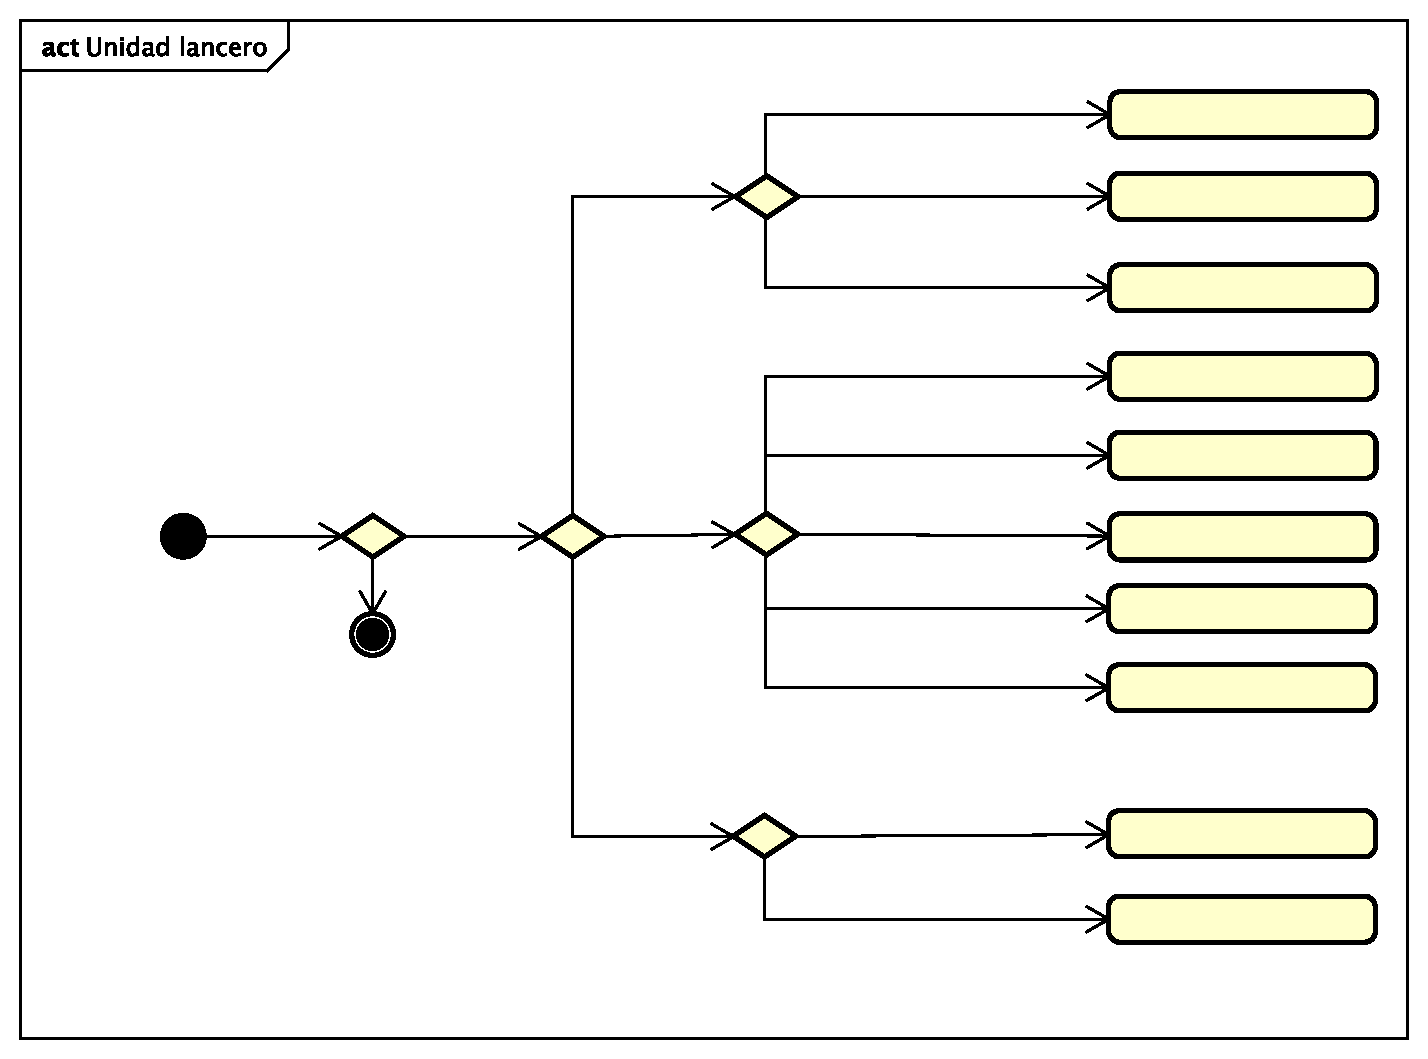
\includegraphics{behaviourTrees/pdfs/arbolLancero}};
            \node (1) at (-6.3,-0.75) {No};
            \node (2) at (-4.9,0.2) {Sí};
            \node (3) at (-6.5,0.3) {¿Vivo?};
            \node (4) at (-3.3,0.4) {¿Estado?};
            \node (5) at (-1.3,6) {Guerra Total};
            \node (6) at (-1.3,0.2) {Ataque};
            \node (7) at (-1.3,-4.9) {Defensa};
            
            \node (8) at (3,6) {¿En base enemiga?};
            \node (9) at (3,7.3) {¿Enemigo cerca?};
            \node (10) at (9,5.6) {Capturar base enemiga};
            \node (11) at (9,7) {Atacar enemigo};
            \node (12) at (9,4.1) {Ir a la base enemiga};
            
            \node (13) at (3,2.9) {¿Enemigo cerca?};
            \node (14) at (3.2,0.2) {¿En base enemiga?}; 
            \node[text width = 4.35cm] (14) at (3.75,1.6) {¿En el punto de curación y pocos puntos de vida?}; 
            \node (16) at (3,-1.1) {¿Pocos puntos de vida?};
            \node (17) at (9,1.25) {Curarse};
            \node (18) at (9,2.6) {Atacar enemigo};
            \node (19) at (9,-2.7) {Ir a la base enemiga};
            \node (20) at (9,-0.1) {Capturar base enemiga};
            \node (21) at (9,-1.35) {Ir al punto de curación};
            
            \node (22) at (3,-4.9) {¿Enemigo cerca?};
            \node (23) at (9,-5.15) {Atacar enemigo};
            \node (24) at (9,-6.6) {Defender};
        \end{tikzpicture}
    }
    \caption{Árbol de comportamiento de lancero}
    \label{fig:lancer}
\end{figure}

\subsubsection{Arquero}
Para la unidad de tipo arquero, hemos ideado que sea una unidad "cobarde", esta prioriza su vida antes que el trabajo en equipo. A diferencia de las otras unidades esta en el \textbf{modo ataque} buscará atacar y capturar la base enemiga, pero siempre que su vida baje peligrosamente huirá a curarse. En el \textbf{modo defensa} también encontramos esta característica, si la unidad se ve muy dañada, irá a curarse a diferencia de las anteriores unidades que simplemente defendían.

\begin{figure}[H]
    \centering
    \resizebox{0.9\textwidth}{!}{
        \begin{tikzpicture}
            \node (0) {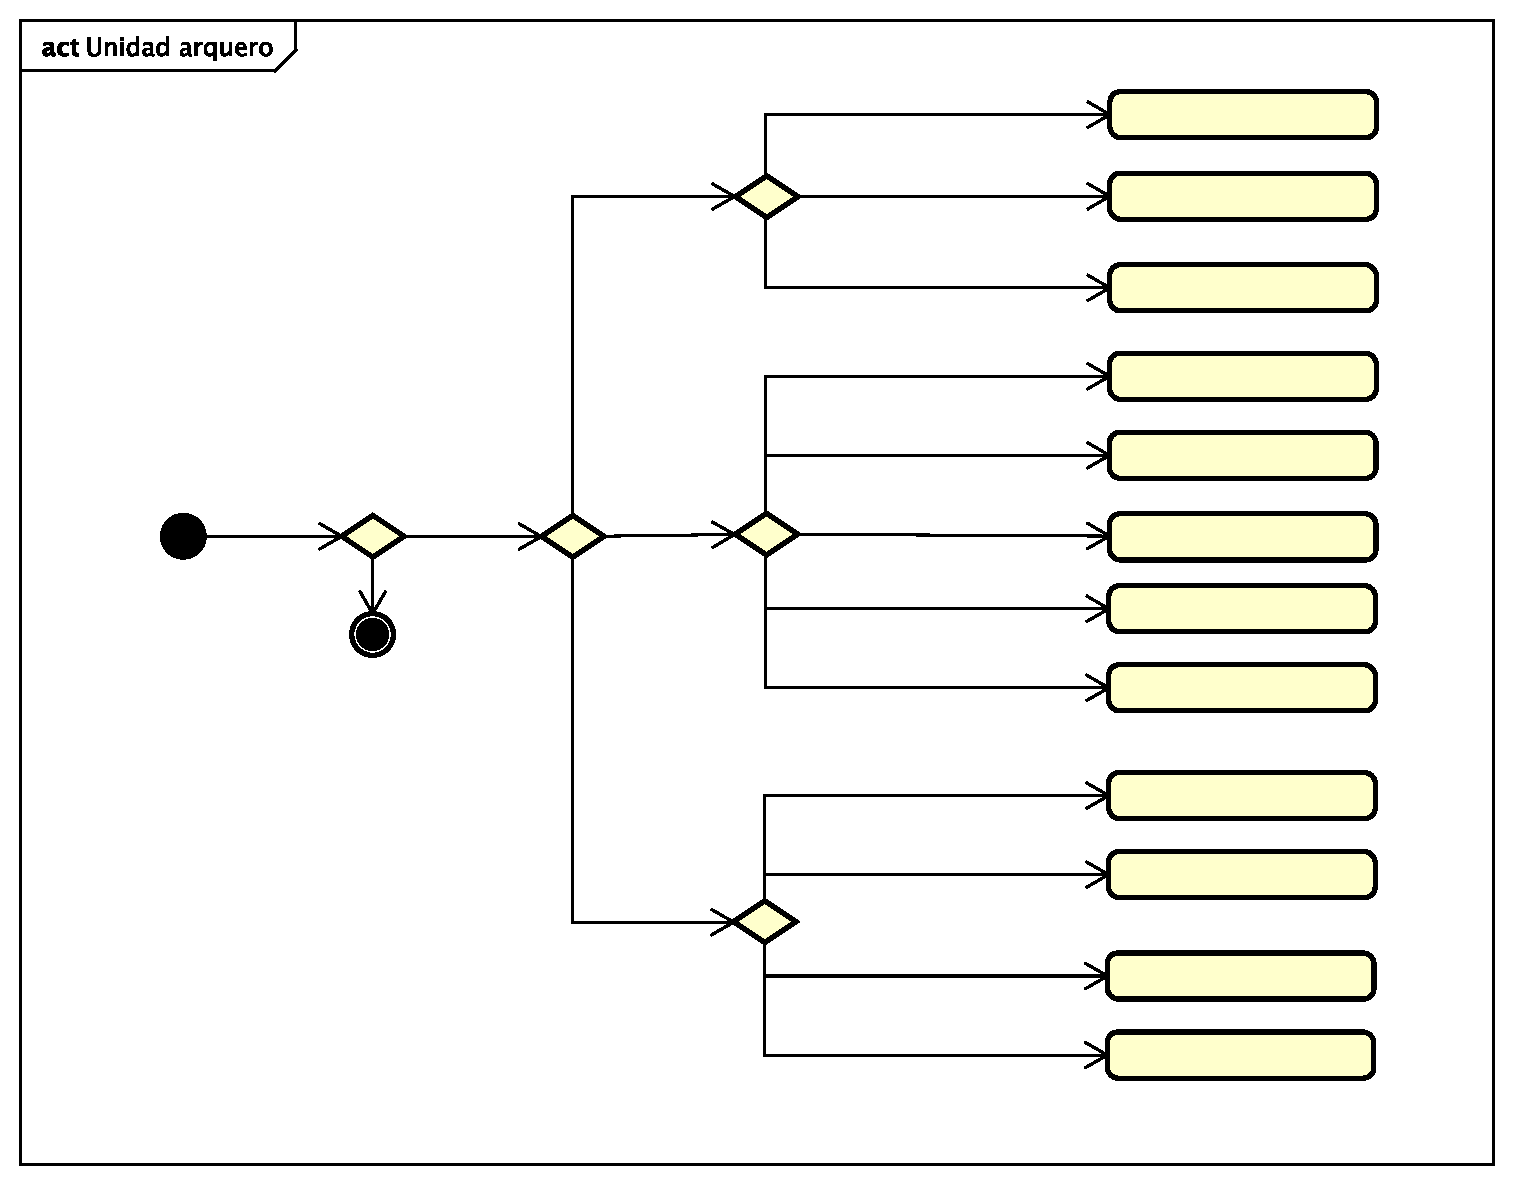
\includegraphics{behaviourTrees/pdfs/arbolArquero}};
            \node (1) at (-6.9,0.35) {No};
            \node (2) at (-5.5,1.2) {Sí};
            \node (3) at (-7.3,1.3) {¿Vivo?};
            \node (4) at (-4,1.4) {¿Estado?};
            \node (5) at (-2,7) {Guerra Total};
            \node (6) at (-2,1.2) {Ataque};
            \node (7) at (-2,-5.3) {Defensa};
            
            \node (8) at (3,7) {¿En base enemiga?};
            \node (9) at (3,8.3) {¿Enemigo cerca?};
            \node (10) at (8.2,6.6) {Capturar base enemiga};
            \node (11) at (8.2,8) {Atacar enemigo};
            \node (12) at (8.2,5.1) {Ir a la base enemiga};
            
            \node (13) at (3,1.2) {¿Enemigo cerca?};
            \node (14) at (3.2,0) {¿En base enemiga?}; 
            \node[text width = 4.35cm] (14) at (3,4) {¿En el punto de curación y pocos puntos de vida?}; 
            \node (16) at (3,2.6) {¿Pocos puntos de vida?};
            \node (17) at (8.2,3.7) {Curarse};
            \node (18) at (8.2 ,0.9) {Atacar enemigo};
            \node (19) at (8.2 ,-1.6) {Ir a la base enemiga};
            \node (20) at (8.2, -0.3) {Capturar base enemiga};
            \node (21) at (8.2, 2.3) {Ir al punto de curación};
            
            \node (22) at (3, -4.5) {¿Pocos puntos de vida?};
            \node[text width = 4.35cm] (23) at (3,-3.2) {¿En el punto de curación y pocos puntos de vida?}; 
            \node (24) at (3, -6.2) {¿Enemigo cerca?};
            \node (25) at (8.2, -6.5) {Atacar enemigo};
            \node (26) at (8.2, -7.8) {Defender};
            \node (25) at (8.2, -3.4) {Curarse};
            \node (26) at (8.2, -4.8) {Ir al punto de curación};
        \end{tikzpicture}
    }
    \caption{Árbol de comportamiento de arquero}
    \label{fig:archer}
\end{figure}

\subsubsection{Caballería} 
Esta unidad la podríamos considerar la mas distintas. de las 4. Su comportamiento se basa en desplazarse en modo de "patrulla" yendo y viniendo a la base. Irá compronbando que se aleje demasiado de su base para volver, y si se encuentra a cualquier enemigo le atacará. Este comportamiendo lo mantendrá siempre que esté \textbf{modo ataque} y en \textbf{modo defensa}. Pero si le ponemos \textbf{modo guerra total} simplemente atacara la base. Cabe recalcar que esta unidad al centrarse en patrullar, nunca llegará a atacar la base enemiga, ni a defender su propia base.

\begin{figure}[H]
    \centering
    \resizebox{0.9\textwidth}{!}{
        \begin{tikzpicture}
            \node (0) {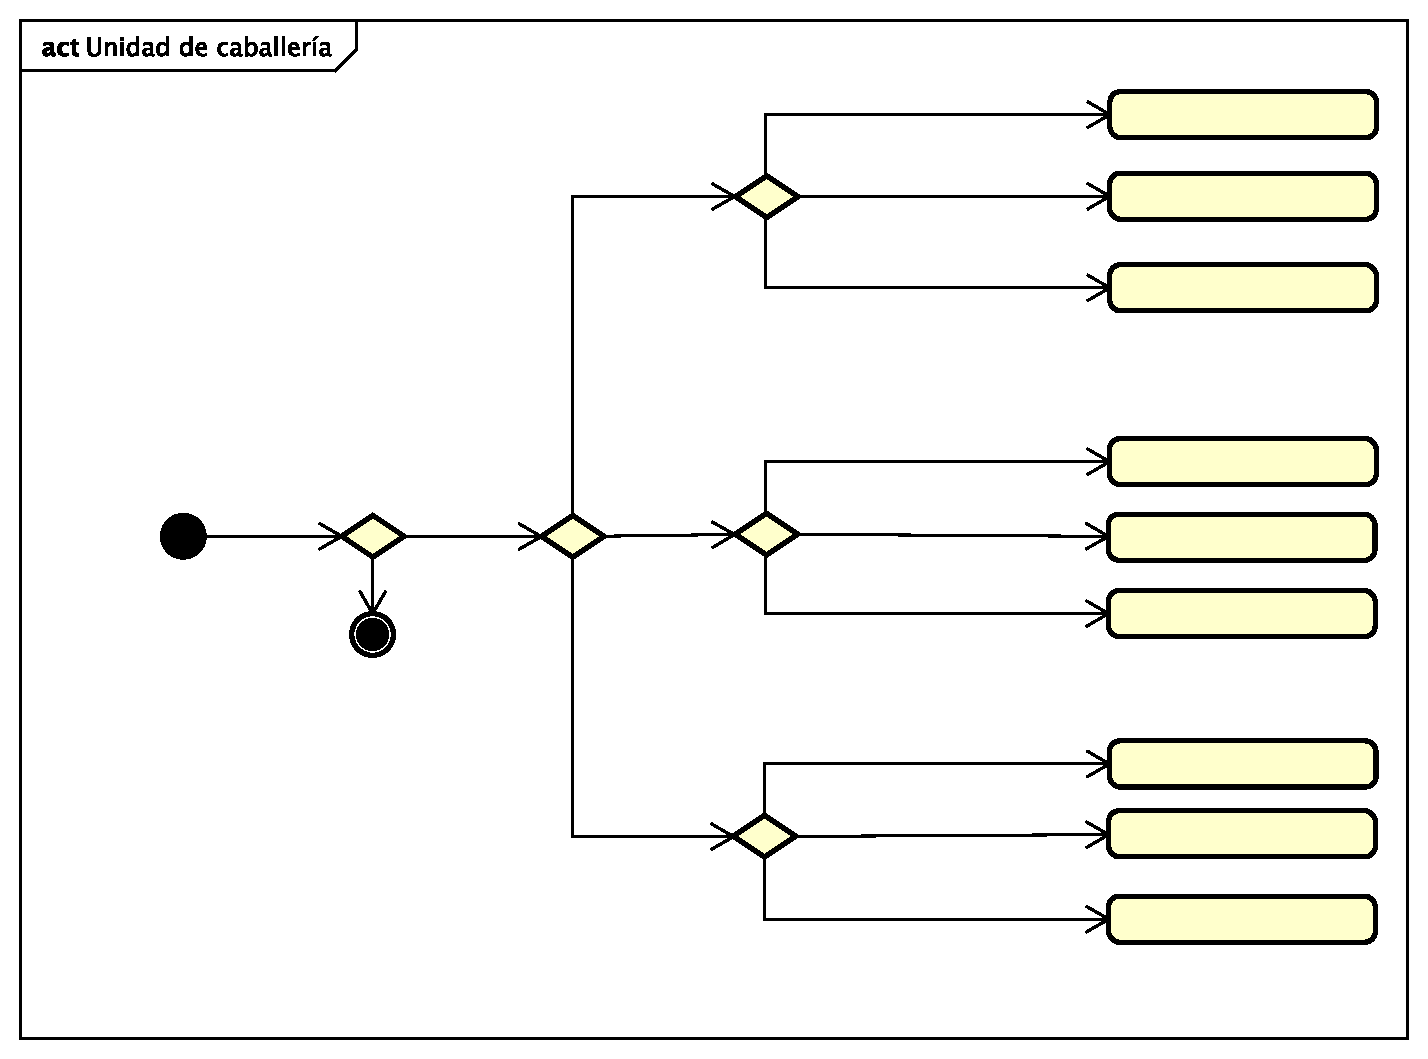
\includegraphics{behaviourTrees/pdfs/arbolCaballo}};
            \node (1) at (-6.3,-0.75) {No};
            \node (2) at (-4.9,0.2) {Sí};
            \node (3) at (-6.5,0.3) {¿Vivo?};
            \node (4) at (-3.3,0.4) {¿Estado?};
            \node (5) at (-1.3,6) {Guerra Total};
            \node (6) at (-1.3,0.2) {Ataque};
            \node (7) at (-1.3,-4.9) {Defensa};
            
            \node (8) at (3,6) {¿En base enemiga?};
            \node (9) at (3,7.3) {¿Enemigo cerca?};
            \node (10) at (9,5.6) {Capturar base enemiga};
            \node (11) at (9,7) {Atacar enemigo};
            \node (12) at (9,4.1) {Ir a la base enemiga};
            
            \node (14) at (3.75,1.5) {¿Lejos de la base?}; 
            \node (17) at (9,1.25) {Defender};
            \node (21) at (9,-1.4) {Ir a la base enemiga};
            
            \node (22) at (3,-3.7) {¿Enemigo cerca?};
            \node (23) at (9,-3.9) {Atacar enemigo};
            \node (25) at (3,-4.9) {¿Lejos de la base?};
            \node (26) at (9,-5.15) {Defender};
            \node (24) at (9,-6.6) {Ir al punto de curación};
        \end{tikzpicture}
    }
    \caption{Árbol de comportamiento de caballería}
    \label{fig:horse}
\end{figure}
